\documentclass[a4paper,12pt]{article}
\hbadness=10000 % prevent stupid useless warnings

\renewcommand{\labelenumii}{\theenumii}
\renewcommand{\theenumii}{\theenumi.\arabic{enumii}.}

\usepackage{silence}
\usepackage[utf8]{inputenc} % Supporto per caratteri UTF-8
\usepackage[T1]{fontenc} % Migliore codifica dei font
\usepackage{lmodern} % Font leggibili
\usepackage{multirow,tabularx}
\usepackage{geometry}
\usepackage{float} % La flag H nelle figure, 
\usepackage{xcolor} % Per i colori
\usepackage{hyperref} % Collegamenti ipertestuali
\usepackage{array} % vertical alignment
\usepackage{graphicx}
\usepackage{titling}
\usepackage{fancyhdr}
%\usepackage{cmbright}

\hypersetup{
  colorlinks=true,
  linkcolor=blue,
  urlcolor=blue,
  pdftitle={},
  pdfauthor={},
  pdfsubject={}
}

\geometry{
  a4paper,
  total={170mm,257mm},
  left=20mm,
  top=20mm,
}

\author{Umberto Frega, Leonardo Napoli}
\setlength{\headheight}{14.49998pt}
\setlength{\footskip}{47.26675pt}
\addtolength{\topmargin}{-0.49998pt}

\fancyhf{}
\fancyfoot[R]{
\includegraphics[width=1.5cm]{assets/logo.png}}
\fancyhead[L]{OPCal}
\fancyhead[R]{\theauthor}

\begin{document}\pagestyle{fancy}

\begin{titlepage}
  \centering
  {\Large \bfseries Progetto di MODULO 2: Laboratorio di Sistemi Informativi\par}
  {\Large Anno Accademico 2024/2025 \par}
  \vspace{1cm} % Adjust if necessary
  \vfill
  {\huge Sistema Informativo per l'Organizzazione Postale Calabrese\par}
  \vfill
  \noindent
  \begin{minipage}[t]{0.5\textwidth}
    \raggedright
    Docente \\  prof. Francesco Parisi
  \end{minipage}%
  \hfill
  \begin{minipage}[t]{0.4\textwidth}
    \raggedleft
    Studenti \\ Umberto Frega 239527 \\ Leonardo Napoli 234364
  \end{minipage}

\end{titlepage}
\tableofcontents
\newpage
\section{Introduzione}
L'Organizzazione Postale Calabrese (OPCal) affiliato a Poste Italiane, con sede legale a Cosenza e filiale a Rende(CS), 
consiste in un Ufficio atto alla spedizione e ricezione di corrispondenze.
\subsection{Sede}
La sede di Rende(CS) in via Marconi, 11 è una piccola struttura avente 3 sportelli e un magazzino. La sua clientela è composta 
prevalentemente da studenti della vicina Università della Calabria che effettuano operazioni di ricevimento pacchi.
La fondazione dell'ufficio risale al 2017, pertanto l'attuale sistema informativo è datato.
\subsection{Organizzativo}
Il direttore dal 2020 è il sig.Lucio Dalla. L'ufficio è diviso in 3 sezioni, la sezione Sportello con 3 dipendenti è gestita 
dal sig.Francesco de Gregori, la sezione Magazzino con 2 dipendenti è gestita dal sig.Adriano Celentano e la sezione Recapiti 
è gestita dal sig.Francesco Guccini con 2 dipendenti al suo seguito. In totale l'organizzazione ammonta a 11 dipendenti.
\begin{figure}[h]
  \centering
  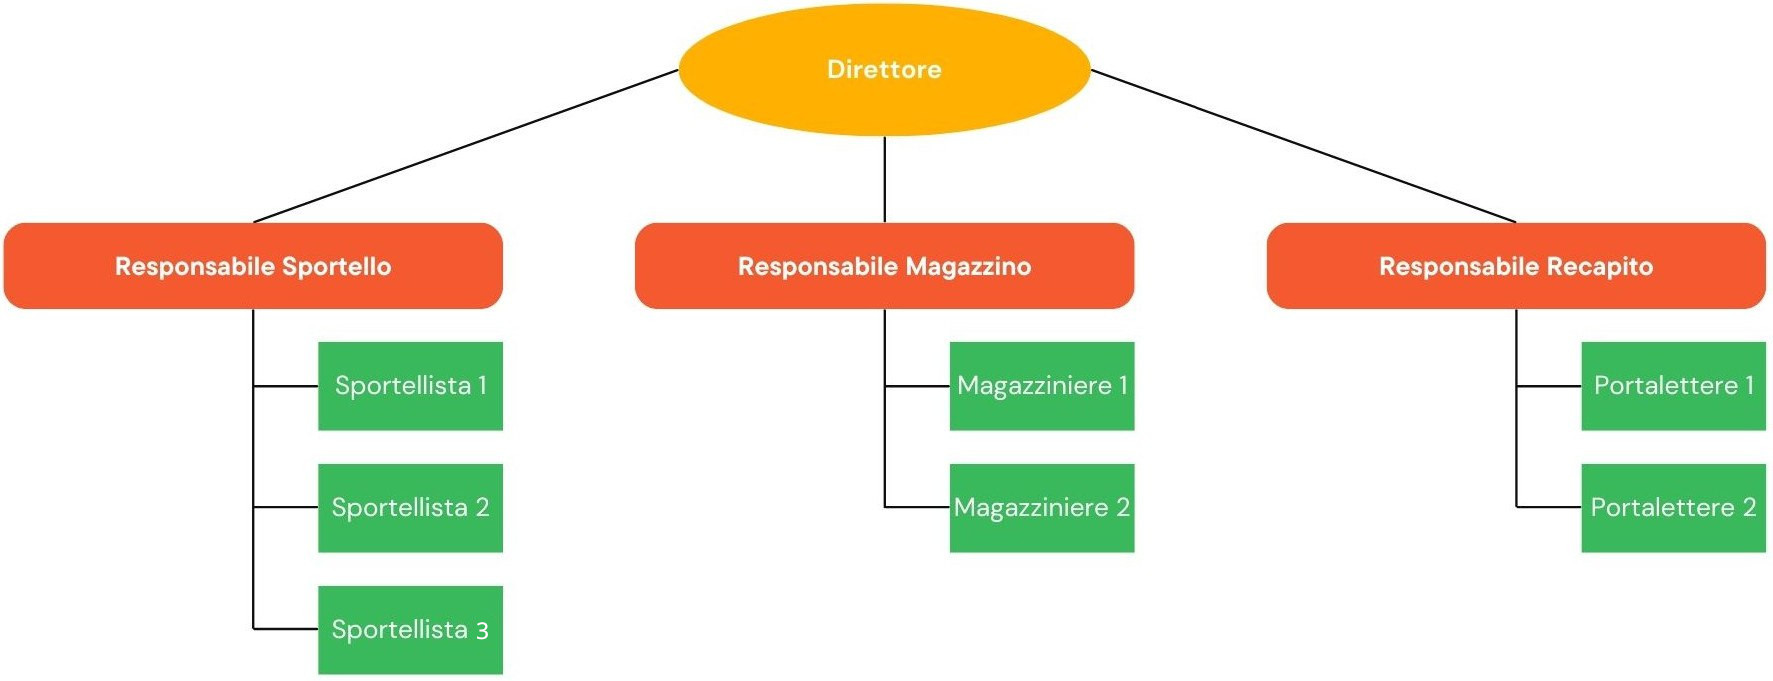
\includegraphics[width=0.8\linewidth]{assets/organigramma.jpg}
  \caption{Organigramma}
\end{figure}
\subsection{Posizione nel Mercato}
L'OPCal detiene ad oggi gran parte del palcoscenico postale cosentino, i competitor sono per la maggioranza servizi privati in rapida ascesa.
\subsection{Prospettive Future}
Nel breve termine l'obiettivo della OPCal rimane il mantenere le quote di mercato nell'area metropolitana cosentina con uno sguardo 
verso l'esterno, con la possibilità a medio/lungo termine di espandere il proprio mercato all'intera area calabrese, continuando a 
garantire una politica di serietà e velocità nel servizio e disponibilità del personale.
\subsection{Benefici Attesi}
L'implementazione del sistema all'interno dell'organizzazione aziendale porterà diversi benefici, come:
\begin{itemize}
  \item Rinnovamento del sistema attuale;
  \item Centralizzazione delle funzionalità;
  \item Centralizzazione dei dati;
  \item Rimozione della dipendenza da documenti cartacei;
  \item Maggiore possibilità di estensione dell'organizzazione;
  \item Semplificazione e deburocratizzazione della user experience;
  \item Possibilità di avere un sistema pubblicitario più esteso ed efficiente tramite il sito web;

\end{itemize}
\subsection{Funzionalità}
Le macro-funzionalità fornite dal sistema infomativo sono le seguenti:
\begin{enumerate}
  \item \textbf{Gestione dei Clienti} \begin{itemize}
      \item Il sistema avrà la funzionalità di mantenere, organizzare e visualizzare le informazioni riguardanti i clienti, 
        quali \textit{spedizioni a carico}, \textit{saldo corrente} e \textit{pacchi in arrivo}.
      \item Ogni cliente avrà la possibilità di visualizzare i suoi dati, prenotarsi allo sportello e prenotare una spedizione 
        tramite l'apposito sito web oppure l'applicativo per dispositivi mobile.
      \item L'utente potrà gestire il proprio saldo corrente e decidere come utilizzarlo.
    \end{itemize}
  \item \textbf{Gestione dei Dipendenti} \begin{itemize}
      \item Il sistema terrà traccia dei vari dipendenti e delle operazioni che svolgono durante il giorno, nonchè dei loro 
        turni e delle loro buste paga.
      \item Il responsabile di ciascun settore potrà visualizzare le prestazioni dei propri subordinati, allo scopo di 
        ammonire e/o premiare i dipendenti meritevoli tramite un sistema di punti.
      \item Ogni dipendente potrà accedere alle informazioni riguardanti la propria busta paga e i turni che dovrà rispettare.
    \end{itemize}
  \item \textbf{Gestione dei Recapiti} \begin{itemize}
      \item Il sistema terrà traccia dello stato delle spedizioni prenotate, in corso ed effettuate in una base di dati.
      \item La base di dati interagirà con l'interfaccia fornita ai dipendenti che si occuperanno di aggiornare lo stato 
        delle spedizioni.
      \item Per ogni missiva presa in carico il sistema sarà responsabile di associarle un codice identificativo univoco a 
        6 cifre che contraddistinguerà l'oggetto dall'inizio alla fine della sua lavorazione,
    \end{itemize}
  \item \textbf{Gestione del Magazzino} \begin{itemize}
      \item Il magazzino interagirà con il sistema tramite una base di dati.
      \item La gestione del magazzino sarà strettamente legata alla gestione dei recapiti, in quanto il magazzino contiene 
        le corrispondenze in entrata e in uscita.
      \item Sarà possibile gestire ogni missiva tramite il codice e trovarla facilmente nonchè catalogarla in base ai suoi dati.
      \item Per ogni oggetto nel magazzino sarà anche memorizzata la sua posizione negli scaffali.
    \end{itemize}
  \item \textbf{Gestione Pagamenti} \begin{itemize}
      \item Il sistema avrà la funzione di monitoraggio dei pagamenti verso l'azienda OPCal.
      \item Il cliente potrà visualizzare lo stato dei propri pagamenti.
    \end{itemize}
  \item \textbf{Interfaccia} \begin{itemize}
      \item Il sistema provvede un'interfaccia per utenti e dipendenti.
      \item Tale interfaccia avrà una duplice implementazione, un sito web e un applicativo per dispostivi mobili (Android o IOS).
      \item Le funzionalità esposte al pubblico saranno tutte disponibili tramite le interfacce specificate.
    \end{itemize}
\end{enumerate}

\newpage
\section{Analisi dei Requisiti}
\subsection{Analisi dello scenario}

\begin{center}
  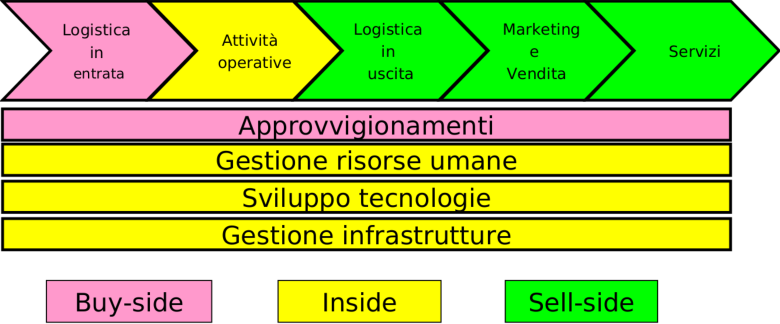
\includegraphics[width=0.8\linewidth]{assets/valueChain.png}
  \vspace{1cm}

  \newcolumntype{Y}{@{}>{\centering\arraybackslash}X @{}}
  \newcolumntype{R}{@{}>{\raggedright\arraybackslash}X @{}}

  \begin{tabularx}{\textwidth}{|*{5}{Y|}}
    \hline
    \textbf{Logistica in entrata (LE)} & \textbf{Attività operative (AO)} & \textbf{Logistica in uscita (LU)} & \textbf{Marketing e vendita (MV)} & \textbf{Servizi post-vendita (SPV)} \\ \hline

    \begin{tabular}{R}
      \hline
      LE1: registrazione cliente               \\ \hline
      LE2: aggiornamento dati cliente          \\ \hline
      LE3: registrazione operazioni dipendenti \\ \hline
      LE4: registrazione spedizioni in entrata \\ \hline
      LE5: registrazione pagamento             \\ \hline
      LE6: controllo magazzino                 \\ \hline
    \end{tabular} &

    \begin{tabular}{R}
      \hline
      AO1: invio corrispondenza                   \\ \hline
      AO2: monitoraggio spedizione                \\ \hline
      AO3: smistamento corrispondenza in arrivo   \\ \hline
      AO4: selezione spedizioni in uscita         \\ \hline
    \end{tabular} &

    \begin{tabular}{R}
      \hline
      LU1: notifica spedizione \\ \hline
      LU2: consegna a cliente  \\ \hline
      LU3: consegna ricevuta   \\ \hline
      LU4: pagamento corriere  \\ \hline
    \end{tabular} &

    \begin{tabular}{R}
      \hline
      MV1: incasso allo sportello   \\ \hline
      MV2: incasso con contrassegno \\ \hline
      MV3: comunicazione promozioni \\ \hline
    \end{tabular} &

    \begin{tabular}{R}
      \hline
      SPV1: gestione resi     \\ \hline
      SPV2: gestione reclami  \\ \hline
      SPV3: raccolta feedback \\ \hline
    \end{tabular} \\ 
    \hline

    \multicolumn{5}{|c|}{Approvvigionamenti (AP)}          \\ \hline
    \multicolumn{5}{|c|}{AP1: acquisto consumabili}        \\
    \multicolumn{5}{|c|}{AP2: acquisto nuova attrezzatura} \\
    \hline
    \multicolumn{5}{|c|}{Gestione risorse umane (GRU)}     \\ \hline
    \multicolumn{5}{|c|}{GRU1: gestione turni di lavoro}   \\
    \multicolumn{5}{|c|}{GRU2: gestione buste paga}        \\ 
    \multicolumn{5}{|c|}{GRU3: valutazione dipendenti}     \\
    \hline
    \multicolumn{5}{|c|}{Gestione infrastrutture (GI)}     \\ \hline
    \multicolumn{5}{|c|}{GI1: manutenzione}                \\
    \hline
  \end{tabularx}
\end{center}

\newpage
\subsubsection{Registrazione cliente}
\textbf{Nome processo} (identificativo): Registrazione cliente (LE1) \\
\textbf{Attori coinvolti}: Cliente, Sportellista, Portalettere \\
\textbf{Archivi coinvolti}: Lista clienti, Rubrica degli indirizzi\\ 
\textbf{Descrizione processo}: Un \textbf{cliente} può registrarsi recandosi fisicamente nella sede dell'ufficio e richiedendo l'apposito modulo di registrazione, 
da compilare con: nome, cognome, data di nascita e indirizzo (nel formato Via, CAP, Città, Provincia) e presentando un documento d'identità come patente o carta d'identità. 
Dopo di ciò lo \textbf{sportellista} dovrà premurarsi di controllare la coerenza delle informazioni all'interno del modulo confrontate con quelle dell documento d'identità. 
Lo \textbf{sportellista} inserirà il documento all'interno della \underline{lista degli utenti}, dove all'occorrenza inserirà anche i dati in merito alle spedizioni del \textbf{cliente}, (vedi LE4: registrazioni spedizioni in entrata) e all'interno della \underline{rubrica degli indirizzi} dove un \textbf{portalettere} 
(vedi LU2: consegna a cliente) può attingere per avere informazioni sul cliente a cui deve consengare.  Nel caso in cui il \textbf{cliente} volesse accedere ai 
suoi dati si deve recare in sede e richiederli allo \textbf{sportellista}, che attingerà alla \underline{lista degli utenti}, i dati presenti nella 
\underline{lista degli utenti} sono costantemente aggiornati dagli \textbf{sportellisti} per garantire la loro correttezza e completezza. 
Questi aggiornamenti possono includere modifiche ai dati personali del cliente, come variazioni di indirizzo o recapiti (vedi LE2: aggiornamento dati cliente). \\
\textbf{Processi correlati:}\\LE2,LE4, LU2.\\ \\
\underline{Cosiderazioni dopo l'implementazione del nuovo sistema informativo}: \\ Queste operazioni saranno gestite in automatico tramite l'apposita piattaforma, 
senza che il cliente vada in sede e senza che lo sportellista lo inserisca manualmente nell'archivio.
\begin{figure}[H]
  \centering
  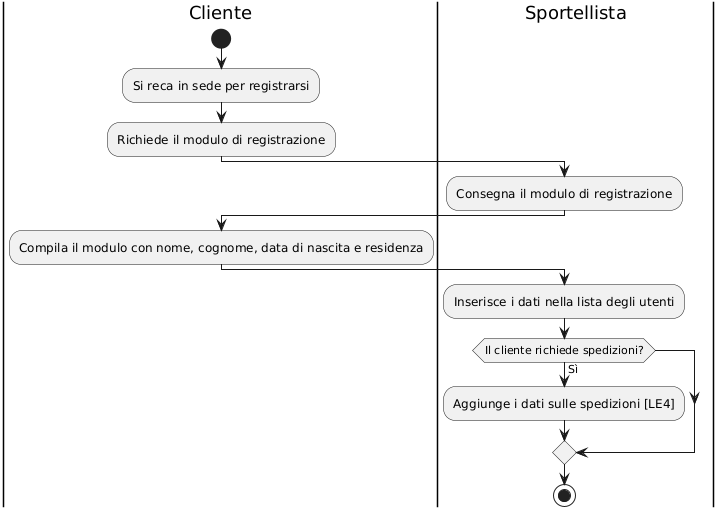
\includegraphics[width=0.8\linewidth]{assets/activitydiagram_LE1.png}
  \caption{Activity Diagram di LE1}
\end{figure}
\begin{figure}[H]
  \centering
  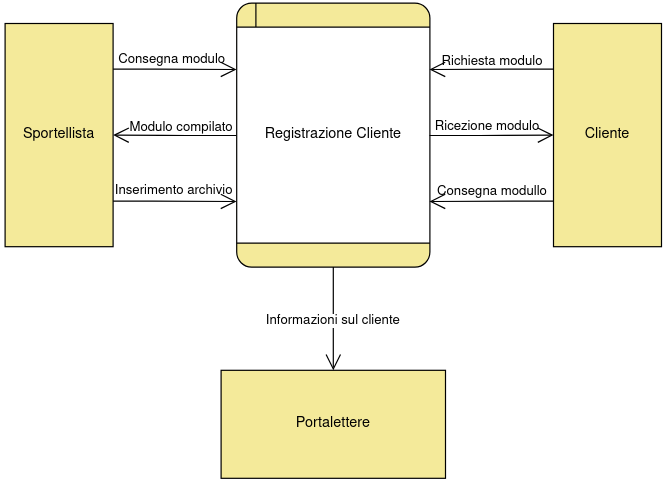
\includegraphics[width=0.7\linewidth]{assets/dataflow_lvl0_LE1.png}
  \caption{Data Flow Diagram LVL 0 di LE1}
\end{figure}
\begin{figure}[H]
  \centering
  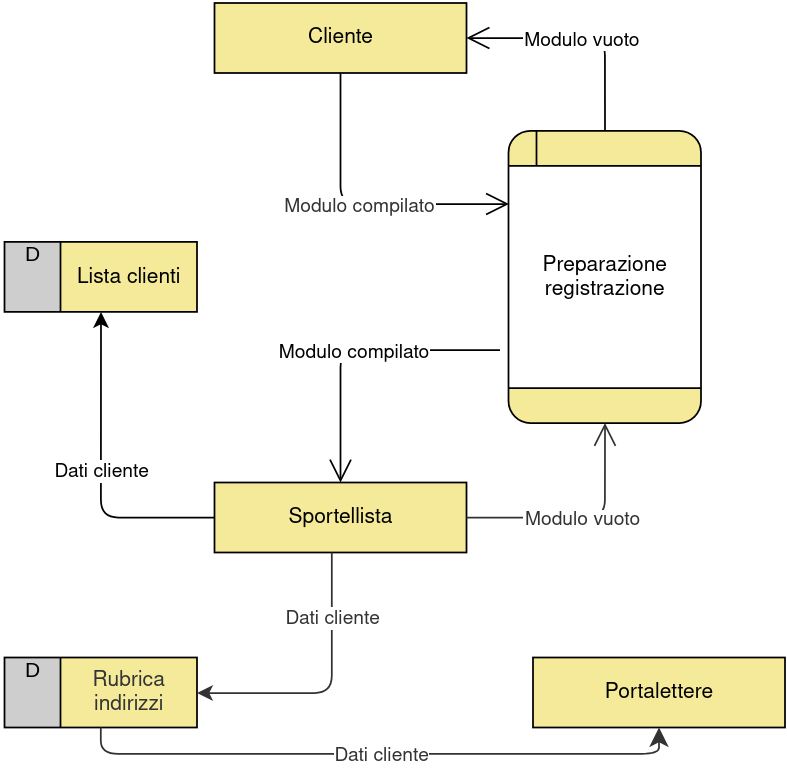
\includegraphics[width=0.7\linewidth]{assets/dataflow_lvl1_LE1.png}
  \caption{Data Flow Diagram LVL 1 di LE1}
\end{figure}

\newpage
\subsubsection{Invio corrispondenza}
\textbf{Nome processo} (identificativo): Invio corrispondenza (AO1) \\
\textbf{Attori coinvolti}: Responsabile magazzino, Magazziniere, Corriere \\
\textbf{Archivi coinvolti}: Registro spedizioni, Inventario, Rubrica corrieri, Lista spedizioni odierne, Registro pagamenti \\
\textbf{Descrizione del processo}: Quando notificato da LE6, il \textbf{responsabile magazzino} controlla nel \underline{registro spedizioni} il numero di articoli
da spedire verso l'esterno. Sceglie un sottoinsieme di articoli (si veda AO4) e compila la \underline{lista spedizioni odierne}, 
nella quale va ad inserire gli articoli da spedire in giornata. Una volta compilata la lista, consulta la \underline{rubrica corrieri} al fine
di trovare quello più conveniente alle condizioni specifiche. Una volta effettuata una stima, inizia a contattare le sedi di corrieri, a partire dalla più 
conveniente, fin quando trova un corriere disponibile in giornata, con il quale concorda un orario per il ritiro ed un prezzo.
Una volta trovato l'accordo con il corriere, compila il documento da mandare al \textbf{direttore}, il quale provvederà al pagamento del \textbf{corriere} (LU4)
e conserverà il documento nel \underline{registro pagamenti}. Il direttore si occuperà inoltre di stampare la ricevuta di pagamento e 
consegnarla ai \textbf{magazzinieri}.
Ricevuta la \underline{lista spedizioni odierne} i \textbf{magazzinieri} consultano l'\underline{inventario}, in cui è riportata la posizione dell'articolo
all'interno del magazzino, e lo mettono da parte, in attesa del \textbf{corriere}. All'arrivo di questo, consegnano la ricevuta e caricano sul furgone gli articoli messi da parte. \\
\textbf{Processi correlati:}\\AO4, LE6, LU4\\
\begin{figure}[H]
  \centering
  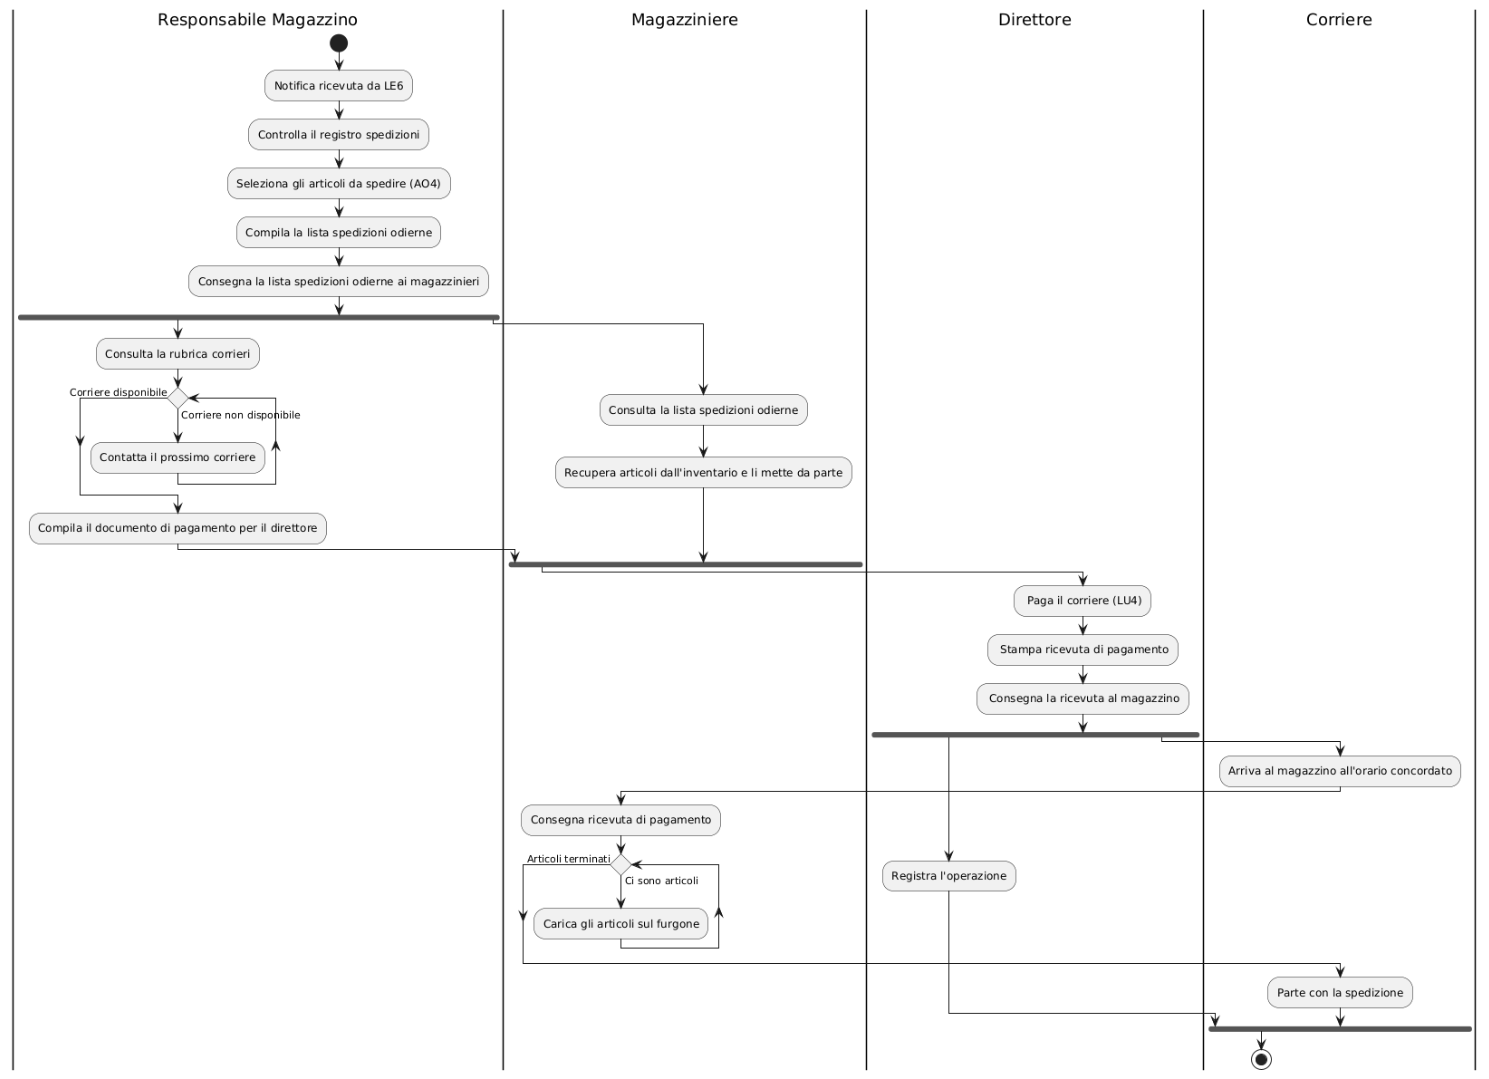
\includegraphics[width=0.8\linewidth]{assets/activitydiagram_AO1.png}
  \caption{Activity Diagram per AO1}
\end{figure}

Si riporta di seguito il dfd di livello 0:
\begin{figure}[H]
  \centering
  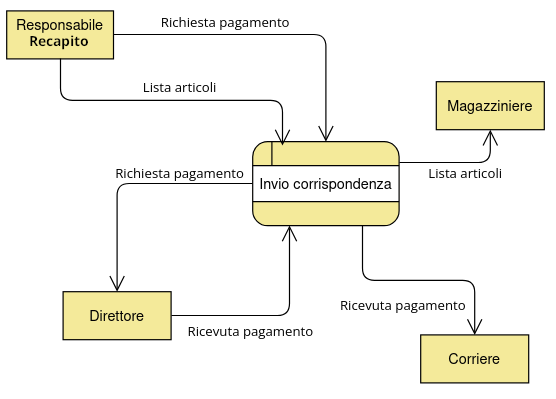
\includegraphics[width=0.8\linewidth]{assets/dfd_0_AO1.png}
  \caption{DFD per AO1}
\end{figure}
Si riporta di seguito il dfd di livello 1:
\begin{figure}[H]
  \centering
  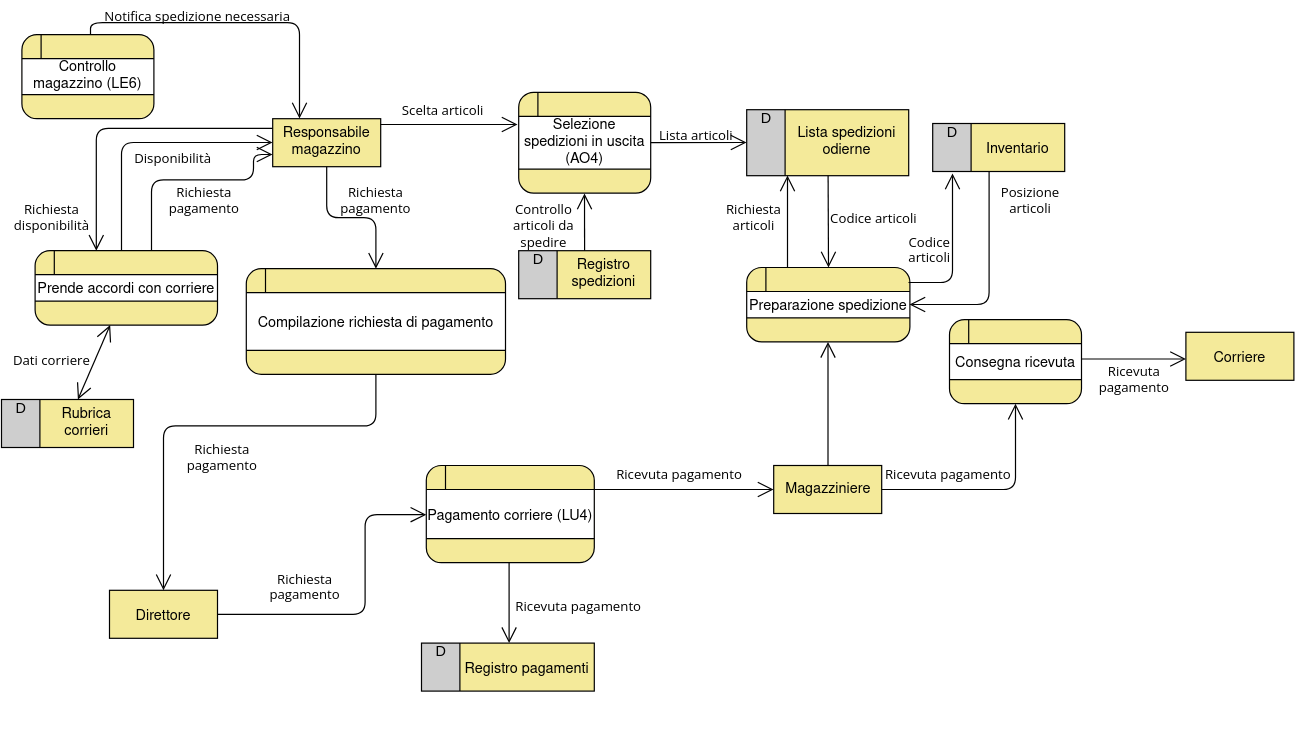
\includegraphics[width=0.8\linewidth]{assets/dfd_1_AO1.png}
  \caption{DFD livello 1 per AO1}
\end{figure}

\subsubsection{Attori e archivi}
\begin{table}[H]
  \centering
  \newcolumntype{Y}{>{\centering\arraybackslash}m{\dimexpr\linewidth/4-2\tabcolsep - 5\arrayrulewidth}}
  \begin{tabularx}{\dimexpr\textwidth-15\arrayrulewidth}{|*{4}{Y|}} %non so perchè ma vuole proprio 15
    \hline
    \textbf{Attore} & \textbf{Descrizione} & \textbf{Processi in cui è coinvolto} & \textbf{Archivi a cui accede} \\ 
    \hline
    Cliente & Uno degli utenti dell'OPCAL & - LE1 & \\ 
    \hline 
    Sportellista & Uno dei dipendenti che lavora nella sezione sportello & -LE1 & \begin{itemize} \item Lista utenti 
    	\item Rubrica degli indirizzi \end{itemize} \\ 
      \hline 
    Portalettere & Uno dei dipendenti che lavora nella sezione corrispondenze & -LE1 & $\bullet$ Rubrica degli indirizzi \\ 
    \hline
    Responsabile magazzino & Il dipendente a capo del magazzino & -AO1 &
    \begin{itemize}
      \item{Registro spedizioni}
      \item{Lista spedizioni odierne}
      \item{Rubrica corrieri}
    \end{itemize} \\
    \hline
    Direttore & Il responsabile generale, si occupa principalmente di contabilità & -AO1 &
    \begin{itemize}
      \item{Registro pagamenti}
    \end{itemize} \\
    \hline
    Magazziniere & Uno dei dipendenti addetto alla sezione magazzino & -AO1 &
    \begin{itemize}
      \item{Lista spedizioni odierne}
      \item{Inventario}
    \end{itemize} \\
    \hline
    Corriere & Un ente esterno che si occupa di gestire la corrispondenza verso zone non sotto la competenza di OPCal & -AO1 & \\
    \hline
  \end{tabularx}
\end{table}

\begin{table}
  \centering
  \newcolumntype{Y}{>{\centering\arraybackslash}m{\dimexpr\linewidth/4-2\tabcolsep - 5\arrayrulewidth}}

  \begin{tabularx}{\dimexpr\textwidth-15\arrayrulewidth}{|*{4}{Y|}} %non so perchè ma vuole proprio 15
    \hline
    \textbf{Archivio} & \textbf{Descrizione} & \textbf{Processi in cui è coinvolto} & \textbf{Attori che vi accedono} \\ \hline
    Lista degli utenti & Archivio in cui sono scritte le informazioni su ogni utente, quali nome, cognome, codice fiscale, e-mail & -LE1 & $\bullet$ Sportellista \\ 
    \hline 
    Rubrica degli indirizzi & Archivio in cui sono scritte informazioni sugli utenti specifiche per i portalettere, queste sono nome, cognome, numero di telefono,
    indirizzo & -LE1 & $\bullet$ Portalettere \\ 
    \hline
    Registro spedizioni & Archivio in cui sono conservate le informazioni delle spedizioni accettate & -AO1 &
    \begin{itemize}
      \item{Sportellista}
      \item{Responsabile magazzino}
    \end{itemize} \\
    \hline
    Inventario & Archivio che testimonia lo stato del magazzino, conservando informazioni sugli articoli in esso presenti & -AO1 &
    \begin{itemize}
      \item{Magazziniere}
    \end{itemize} \\
    \hline
  \end{tabularx}
\end{table}

\newpage
\subsection{Requisiti funzionali}
I gruppi funzionali che si è deciso di implementare sono quelli riguardanti la \textbf{gestione dei clienti} e la \textbf{gestione dei recapiti}.

\subsubsection{Gestione clienti}
\begin{enumerate}
	\item{(MUST)} Implementare una schermata di sign-in [Cliente];
	\item{(MUST)} Inserimento dei propri dati anagrafici[Cliente];
	\item{(MUST)} Modifica dei propri dati anagrafici[Cliente];
	\item{(MUST)} Implementare la possibilità di poter registrare delle spedizioni[Cliente]; 
	\item{(MUST)} Implementare la possibilità di poter tracciare le spedizioni[Cliente];
	\item{(MUST)} Aggiungere una funzione per iniziare una procedura di reso[Cliente];
	\item{(MUST)} Scaricare tutti i documenti da compilare per procedere con il reso[Cliente];
	\item{(MUST)} Poter annullare o modificare una procedura di reso[Cliente];
	\item{(MUST)} Introdurre di un sistema di sicurezza per il login nella piattaforma[Cliente, Sportellista];
	\item{(MUST)} Dare la possibilità di avere uno storico delle consegne[Cliente];
	\item{(MUST)} Introdurre un ordinamento per lo storico delle consegne[Cliente]:
	\begin{enumerate}
		\item Per data, dalla più alla meno recente (Default);
		\item Per tipo di spedizione;
		\item Per numero di ordine;
		\item In ordine alfabetico.
	\end{enumerate} 
	\item{(MUST)} Visualizzare le fatture a proprio carico[Cliente];
	\item {(MUST)} Ordinare la lista delle fatture a proprio carico[Cliente]:
	\begin{enumerate}
		\item Per stato del pagamento (Default);
		\item Per data del pagamento;
		\item In ordine alfabetico;
	\end{enumerate}
	\item{(MUST)} Visualizzare in tempo reale lo stato delle spedizioni di ogni cliente [Sportellista];
	\item{(MUST)} Visualizzare in tempo reale lo stato dei pagamenti di ogni cliente [Sportellista];
	\item{(MUST)} Accedere ai dati anagrafici dei clienti [Sportellista, Portalettere];
	\item{(MUST)} Modificare i dati anagrafici dei clienti [Sportellista];
	\item{(MUST)} Accedere ai dati delle spedizioni dei clienti [Sportellista, Portalettere];
	\item{(MUST)} Modificare i dati in merito alle spedizioni dei clienti [Sportellista, Portalettere];
	\item {(MUST)}  Implementare un sistema di mailing [Sportellista]:
\end{enumerate}

Per il \textbf{Requisito 20, Implementare un sistema di mailing}, si riporta di seguito una descrizione dettagliata: \\
 Attore Principale: Sportellista \\
 Descrizione dello scenario principale:  
 \begin{enumerate}
 \item Un cliente si registra all'interno della piattaforma;
 \item Inserisce nel campo e-mail il suo indirizzo;
 \item Viene creata una \textit{mailing list} e viene inserito all'interno questo cliente;
 \item Comincia una pratica di reso, richiede una spedizione oppure un'appuntamento in sede;
 \item Quando ci sono aggiornamenti su un qualcosa che concerne l'utente viene inviata una e-mail in materia;
 \item Nel caso in cui ci siano informazioni sui servizi dell'organizzazione possono essere mandati aggiornamenti tramite le \textit{newsletter}.
\end{enumerate}

Descrizione di scenari alternativi: \\
SA1 (Non arriva l'email di aggiornamento): 
 \begin{enumerate}
 	\item Viene mandata una seconda e-mail;
 	\item Se il problema persiste si prova a sostituire l'indirizzo dell'utente o a creare una nuova mailing list.
 \end{enumerate} 
Di seguito è riportato il diagramma dei casi d'uso per \textbf{l'Area Funzionale 1: Gestione clienti}, per semplificare la lettura è diviso in due :
\begin{figure}
\centering
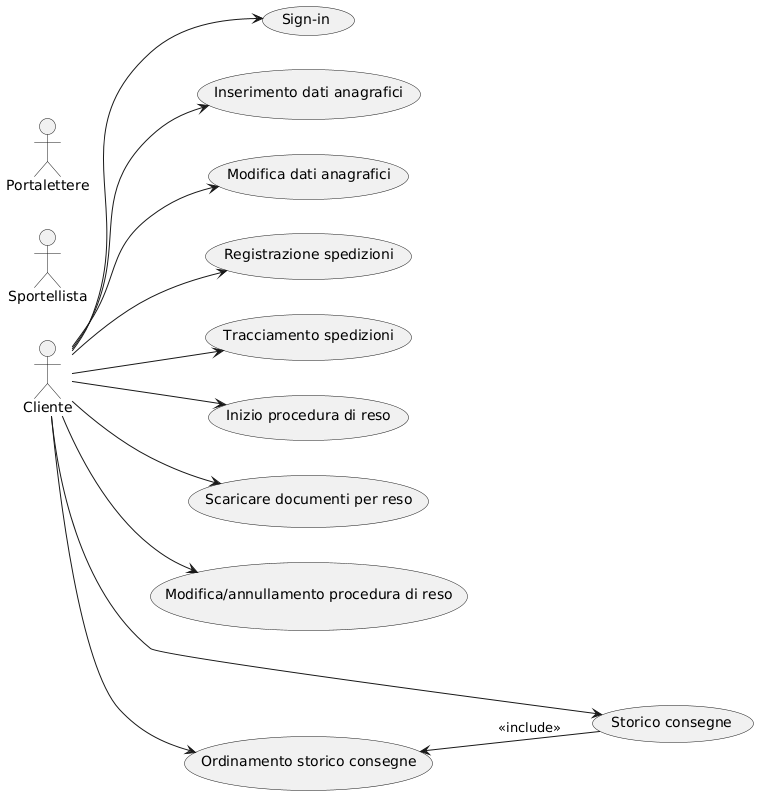
\includegraphics[width=10cm]{assets/usecase_clienti.png}
\caption{Diagramma Casi d'Uso 1}
\end{figure}
\begin{figure}
	\centering
	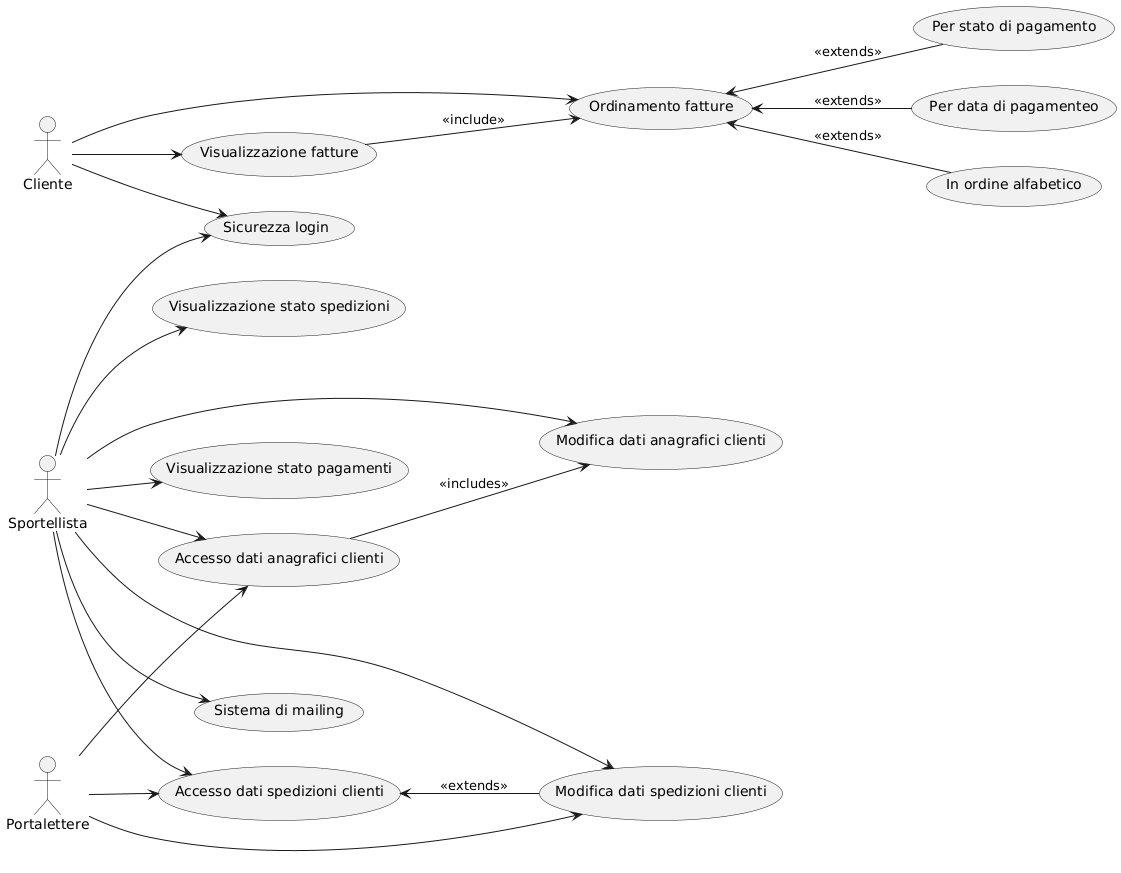
\includegraphics[width=10cm]{assets/usecase_clienti_2.png}
	\caption{Diagramma Casi d'Uso 2}
\end{figure}

\clearpage
\subsubsection{Gestione recapiti}
\begin{enumerate}
  \item{(MUST)} Associare un cliente ai suoi dati rilevanti [sportellista, portalettere];
  \item{(MUST)} Visualizzare gli indirizzi dei clienti [portalettere];
  \item{(MUST)} Visualizzare le spedizioni in arrivo ad un indirizzo [portalettere];
  \item{(MUST)} Visualizzare le spedizioni da ritirare [portalettere];
  \item{(MUST)} Creare una spedizione [sportellista, cliente];
  \item{(MUST)} Distinguere tra spedizioni interne e spedizioni verso l'esterno [magazziniere];
  \item{(MUST)} Tenere traccia delle spedizioni prenotate, in corso ed effettuate [responsabile recapiti];
  \item{(MUST)} Modificare il ciclo di vita di una spedizione(prenotata, in corso, effettuata);
  \item{(MUST)} Prendere in carico una spedizione [sportellista, portalettere];
  \item{(MUST)} Aggiornare lo stato di una spedizione:
    \begin{enumerate}
      \item{Da "prenotata" a "presa in carico" [sportellista, portalettere]};
      \item{Da "presa in carico" a "spedita" [magazziniere]};
      \item{Da "spedita" a "arrivata alla filiale" [magazziniere]};
      \item{Da "arrivata alla filiale" a "in consegna" [magazziniere]};
      \item{Da "in consegna" a "consegnata" [portalettere]};
      \item{Da "in consegna" a "tentato recapito" [portalettere]};
    \end{enumerate}
  \item{(MUST)} Filtrare la lista degli indirizzi, di default ordinata per nome del cliente, secondo i seguenti criteri[portalettere]:
    \begin{enumerate}
      \item{Comune di appartenenza};
      \item{Orario preferito per la consegna};
      \item{Numero di ordini ricevuti};
      \item{Numero di ordini spediti};
      \item{Per data ultimo ordine};
      \item{Per data primo ordine};
    \end{enumerate}
  \item{(MUST)} Filtrare la lista delle spedizioni, di default ordinata per data, secondo i seguenti criteri:
    \begin{enumerate}
      \item{Per pagamento};
      \item{Per indirizzo di consegna};
      \item{Per indirizzo di partenza};
      \item{Per stato della spedizione};
    \end{enumerate}
  \item{(MUST)} Assegnare ad ogni spedizione un codice univoco [magazziniere, portalettere];
  \item{(MUST)} Identificare una spedizione solo tramite il suo codice [magazziniere, portalettere];
  \item{(MUST)} Visualizzare la lista dei corrieri esterni [responsabile magazzino];
  \item{(MAY)}  Aggiornare la lista dei corrieri con i prezzi automaticamente aggiornati [responsabile magazzino];
  \item{(MUST)} Calcolare un preventivo per il corriere esterno selezionato [responsabile magazzino];
  \item{(MUST)} Prenotare il ritiro da parte di un corriere [responsabile magazzino];
  \item{(MUST)} Registrare il pagamento al corriere [direttore]
\end{enumerate}

\textbf{N.B.} \\
Tenere a mente la distinzione tra \textbf{ciclo di vita} e \textbf{stato} di una spedizione. Il \textbf{ciclo di vita} si riferisce
alla situazione della spedizione(prenotata, in corso, effettuata). Per ognuna di queste, la spedizione verrà catalogata in basi di dati differenti.
Lo \textbf{stato} è proprio solo delle spedizioni \textit{in corso}(presa in carico, consegnata, ecc.).
\\ \\
Per il \textbf{caso d'uso 5 (Creare una spedizione)} segue descrizione dettagliata: \\
Una spedizione può essere creata da due attori separati:
\begin{enumerate}
  \item{Sportellista}: nel caso in cui un cliente si rechi in sede per effettuare una spedizione, l'intera operazione viene effettuata dallo sportellista;
  \item{Cliente}: il cliente può creare la spedizione tramite l'interfaccia offerta. In questo caso la spedizione effettuata verrà considerata come \textit{prenotata}
    e il cliente dovrà attendere il ritiro alla prima data utile.
  
\end{enumerate}
Di seguito è riportato il diagramma dei casi d'uso per \textbf{l'Area Funzionale 2: Gestione recapito} :
\begin{figure}[H]
\centering
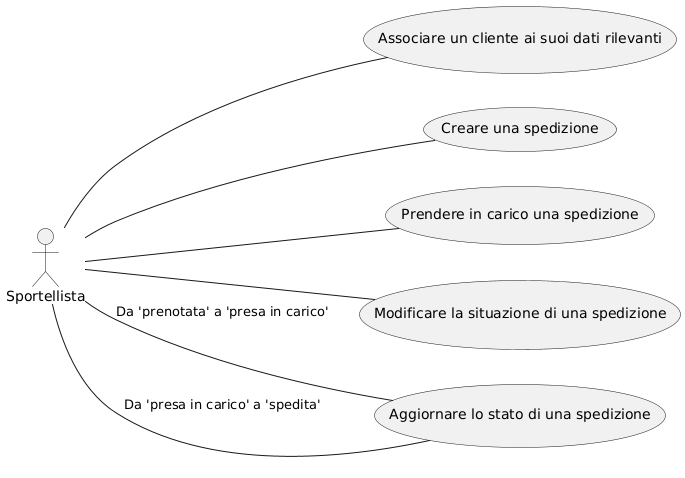
\includegraphics[width=10cm]{assets/usecase_recapito_1.png}
\end{figure}
\begin{figure}[H]
	\centering
	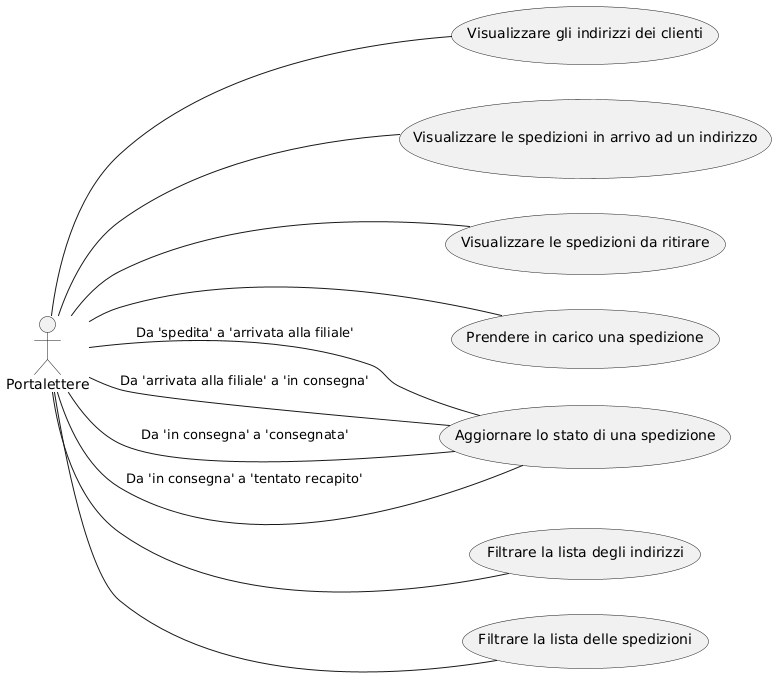
\includegraphics[width=10cm]{assets/usecase_recapito_2.png}
\end{figure}
\begin{figure}[H]
	\centering
	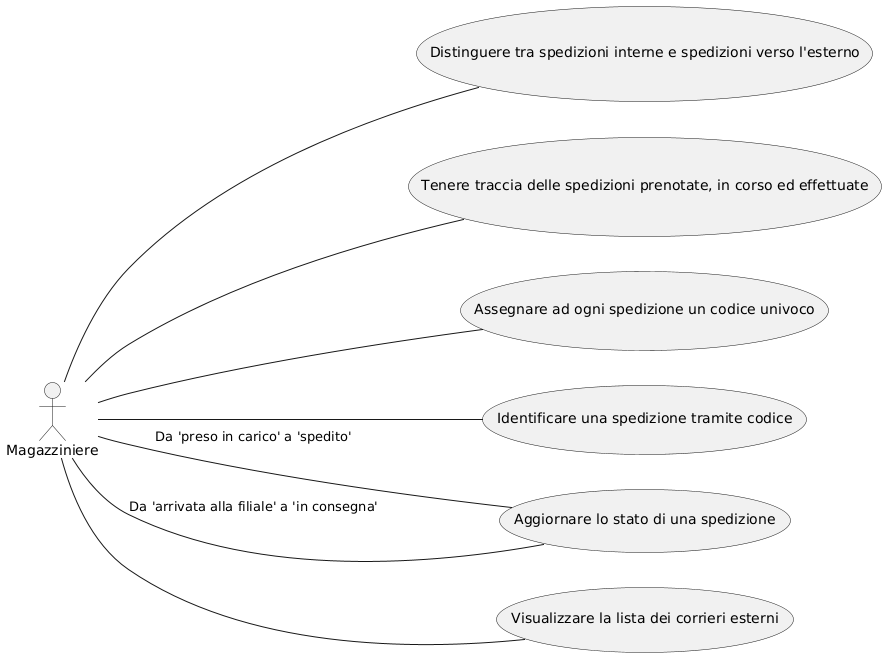
\includegraphics[width=10cm]{assets/usecase_recapito_3.png}
\end{figure}
\begin{figure}[H]
	\centering
	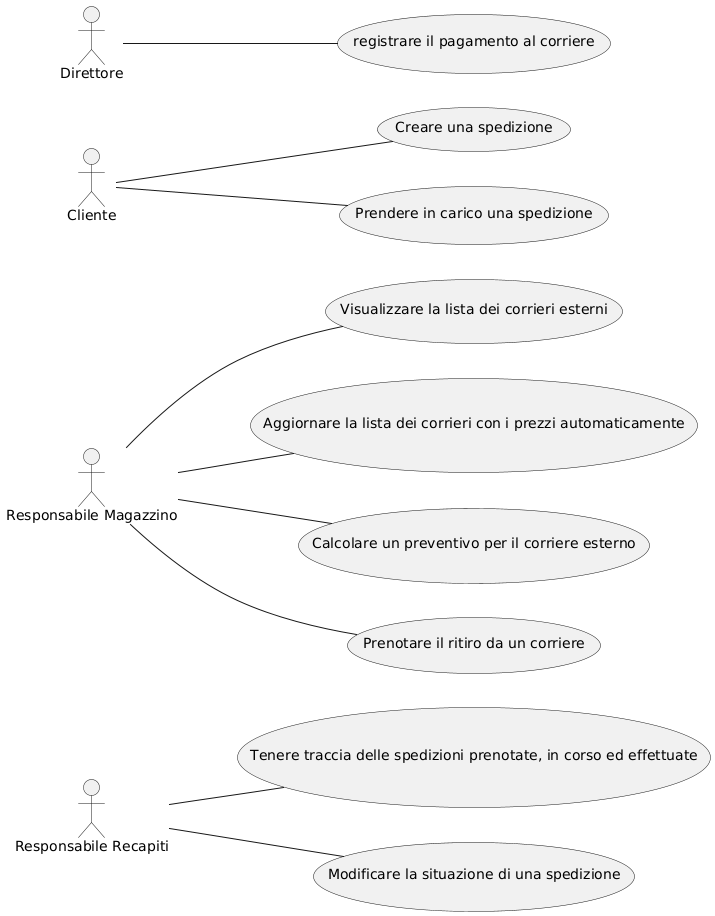
\includegraphics[width=10cm]{assets/usecase_recapito_4.png}
	\caption{Diagramma Casi d'Uso Recapito}
\end{figure}
\end{document}
